\section{Design av l\o  sningen}

	\subsection{Overordnet design (Holger)}
	
		\begin{figure}[h]
		\centering
		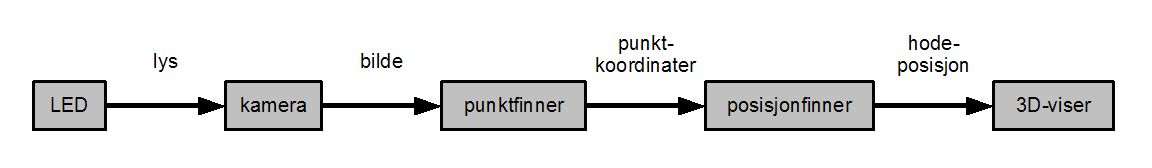
\includegraphics[width=\textwidth]{graphics/main_design.png}
		\caption{Overordnet design}
		\label{fig:main_design}
		\end{figure}
		
		Den overordnede designen er en pipeline som begynner med lys fra LEDs og ender opp med visning av en 3D-scene. Figur \ref{fig:main_design} illustrerer dette. Vi ser at alt begynner med infrar\o  de LEDs som er festet p\aa \space hodet til brukeren. Disse sender lys som filmes av kameraet. Bildene fra kameraet leses av kode som finner punktene p\aa \space bildet som senteret til hvert filmet LED. Disse koordinatene sendes til kode som bruker dem til \aa \space \space beregninge posisjonen til hodet. Denne posisjonen sendes til kode som viser en 3D-scene p\aa \space skjermen, hvor synsvinkelen passer posisjonen til hodet.
	
	\subsection{Design av LED-headset (Jon)}
	
		
	
	\subsection{Design av punktfinneren (Holger)}
	
		Punktfinnerens oppgave er \aa \space lese bildet fra kameraet og finne koordinatene til lyspunktene til LED-ene i dette bildet. Punktfinnerens oppf\o rsel er illustrert i figur \ref{fig:pointfinder_sequence}. Sekvensen er et eksempel p\aa \space typisk oppf\o rsel. Det starter med at finneren s\o ker gjennom hele bildet etter punktenes koordinater (kalt kalibrering). Deretter oppdateres disse koordinatene ved \aa \space kun s\o ke i omr\aa det rundt der punktet var sist. Slik inneholder punktfinneren alltid oppdaterte punktkoordinater. Om punktene ikke finnes kan man kalibrere om igjen.
		
		\begin{figure}[h]
		\centering
		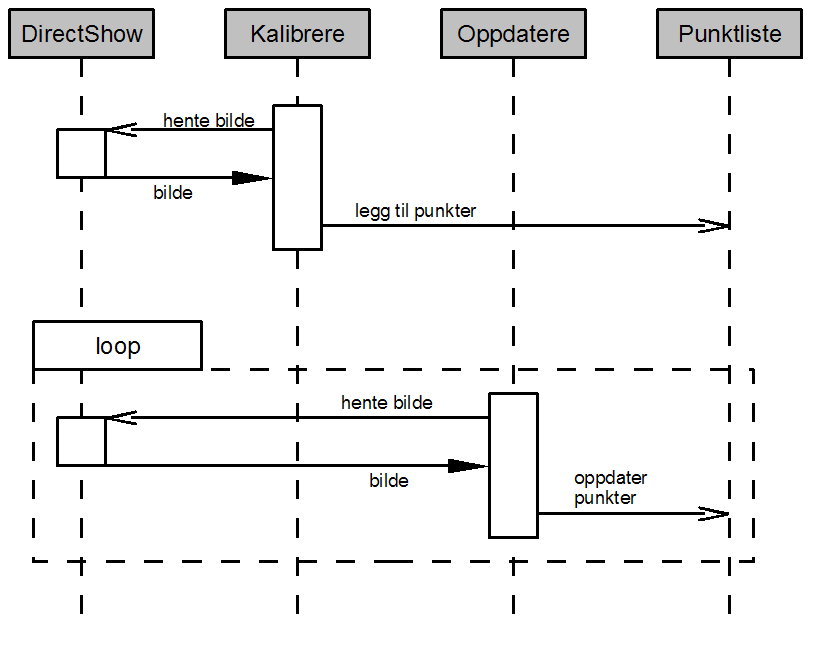
\includegraphics[width=\textwidth]{graphics/pointfinder_sequence.png}
		\caption{Sekvensdiagram for punktfinner}
		\label{fig:pointfinder_sequence}
		\end{figure}
		
		Algoritmen for s\o king gjennom hele bildet (kalibrering) kan utrykkes med f\o lgende pseudokode:
		
		\begin{enumerate}
			\item S\o k i linje etter linje fra topp til bunn i hele bildet etter {\it count\_limit} etterf\o lgende bildepunkter hvis lysintensitet (sum av r\o d-, gr\o nn og bl\aa -farge) er h\o yere enn minstem\aa l {\it intensity\_cutoff}
			\item For hver slik etterf\o lgende rekke som finnes:
				\begin{enumerate}
					\item {\it repr} = siste av de etterf\o lgende bildepunktene
					\item Sjekk om {\it repr}s avstand er mer enn {\it distance\_cutoff} fra alle andre lyspunkter funnet hittil
					\item Hvis den er det, legg til {\it repr} som funnet lyspunkt
				\end{enumerate}
		\end{enumerate}
		
		Algoritmen for oppdatering av punkter som er funnet kan utrykkes med f\o lgende pseudokode:
		
		\begin{enumerate}
			\item For hvert punkt {\it point}:
				\begin{enumerate}
					\item S\o k i linje etter linje i et omr\aa de med radius {\it search\_radius} rundt punktet etter {\it count\_limit} etterf\o lgende bildepunkter hvis lysintensitet er h\o yere enn minstem\aa l {\it intensity\_cutoff}
					\item Om dette blir funnet:
						\begin{enumerate}
							\item {\it repr} = siste av de etterf\o lgende bildepunktene
							\item {\it point} = {\it repr}
						\end{enumerate}
					\item
				\end{enumerate}
		\end{enumerate}
	
	\subsection{Design av posisjonsfinneren og 3D-viseren (Vegar)}
	
		
	
\section{Implementasjon av l\o  sningen}

	\subsection{Valg av kamera}
	
		Kriterier vi ser etter:
		
		\begin{itemize}
			\item Bildebrikke som kan fange opp infrar\o dt lys
			\item Stor n\o yaktighet p\aa \space avstand
			\item St\o tte for live feed til en datamaskin
			\item Manuell fokus
			\item Pris
		\end{itemize}
		
		 
		For \aa \space f\aa \space en fornuftig pris p\aa \space kameraet unders\o kte vi vanlige full hd (high definition) kamera. Vi s\aa \space etter et kamera som fulgte standarden 1080P. Dette er en oppl\o sning p\aa \space 1920 linjer horisontalt, 1080 linjer vertikalt, og gir h\o y n\o yaktighet p\aa \space avstand. P st\aa r for progressive. Det betyr at kameraet tar et fullt bilde i motsetning til interlaced, hvor det bare tar annenhver linje. Vi \o nsker progressive for \aa \space f\aa \space mindre bildebehandling enn ved interlaced. For \aa \space f\aa \space live feed fra kameraet er vi avhengig av \aa \space overf\o re store datamenger fra kameraet til datamaskinen. Analog overf\o ring er ikke aktuelt p\aa \space grunn av kvalitetstapet i bildet. Hver kanal gir ut 1byte per piksel, og det er 3 kanaler for r\o d, gr\o nn og bl\aa . Kameraet gir ut 25 bilder i sekundet, som gir 150 USB 2.0 kan overf\o re opp til 480 megabit, og dette er for lite til \aa \space \o verf\o re en ukomprimert live feed i full oppl\o sning. Derfor er vi avhengige av HDMI output p\aa \space kameraet. En stor del av kameraene tar i bruk en 3CCD bildesensor. CCD brikkene fanger opp en del av det infrar\o de spekteret i tillegg til synlig lys, derfor settes det p\aa \space et infrar\o dt filter foran sensoren. Vi tar utgangspunkt i at vi fjerner dette filteret. Dette vil f\o re til at autofokusen ikke vil fungere lenger, og vi er derfor avhengig av manuell fokus. CMOS bildebrikker er et annet alternativ da disse ogs\aa \space fanger opp infrar\o dt lys.

		Valget av kamera falt til slutt p\aa \space et Panasonic HDC-SD9 kamera. Dette har etter spesifikasjonene 3CCD bildesensor, HDMI utgang, manuell fokus, 1080P bilde og lav pris. Etter noe fram og tilbake fikk vi servicemanualen til kameraet fra Panasonic. Den beskriver trinnvis hvordan IR-filteret kan fjernes. Vi fikk fjernet IR-filteret, men det viste seg at manuell fokus ikke fungerte som forventet. Det var en automatisert funksjon som sto for fokuset, slik at dette ikke kunne stilles inn riktig uten filteret. Optimalt burde vi erstattet filteret med en glassbit, men vi valgte \aa \space erstatte filteret med gjennomsiktig pvc plast, slik at lysbrytningen skulle ligne p\aa \space den gjennom IR-filteret. De optiske egenskapene til plasten er ikke spesielt bra, men vi ender likevel opp med et mye bedre bilde p\aa \space grunn av at bildet ikke lenger er like langt ute av fokus. For v\aa r applikasjon er dette bildet mer enn nok til \aa \space tracke IR lys i rommet. For \aa \space lettere kunne tracke lyset fra dioden har vi tatt i bruk et filter som blokkerer alt lys utenom infrar\o dt. REF: (OPTIR 1.0 NG 305 X 100 fra Instrument Plastics. Kj\o pt via http://www.farnell.com (varenr 177143))
		
	\subsection{Valg av IR-sender}
		
		Kriterier vi ser etter:
	
		\begin{itemize}
			\item Lett \aa \space bruke
			\item Liten vekt
			\item Minst mulig i veien
			\item H\o y intensitet p\aa lyset
		\end{itemize}

		M\aa let var \aa \space finne en l\o sning som ikke er i veien for brukeren. Optimalt sett s\aa \space trenger ikke brukeren ta p\aa \space seg noe ekstra utstyr. For \aa \space kunne tracke brukeren trengs det minimum to lyskilder og 1 kamera, eller to kamera og en lyskilde. Vi bestemte oss for \aa \space bruke et tr\aa dl\o st headset, da dette ikke er spesielt tungvindt \aa \space ha p\aa . Dette har ogs\aa \space et innebygd batteri som vi kan koble lyskilder p\aa . For \aa \space kunne skille rotasjon fra avstand trengs det en tredje diode. Denne kan festes p\aa \space mikrofonen.

		Vi gikk til innkj\o p av et Logitech Clearchat tr\aa dl\o st headset, og 3 IR dioder med h\o y intensitet. REF STUFF CHECK MED ANDERE GRP! IR diodene var spesifisert til \aa \space t\aa le opp mot 1 Ampere ???? Skjekk opp. Batteriet p\aa \space headsettet gir ut 3,7V. M\aa let var \aa \space f\aa \space mest mulig intensitet ut, slik at lyset er synlig lengst mulig bort, og slik at dioden ikke trenger peke direkte p\aa \space kameraet for \aa \space kunne registreres. Diodene vil fungere som en kortslutning om de festes rett p\aa \space batteriet, s\aa \space for \aa \space begrense str\o mmen gjennom dem trengs det motstand i serie. Vi dimensjonerte oppsettet, med en motstand p\aa \space 47? foran dioden, slik at det g\aa r under 100mA gjennom hver diode.

		Det viste seg at kameraet klarte \aa \space detektere diodene bedre enn forventet, som gj\o r at diodestr\o mmen er kraftig overdimensjonert, noe som g\aa r hardt utover batterikapasiteten til headsettet.
